\documentclass[a4paper,12pt]{article}
\usepackage{amsmath}
\usepackage{graphicx}
\usepackage{bm}

\graphicspath{ {.} }
\begin{document}

\title{%
  The process of minimizing the error function within Machine Learning \\
  \small Mathematics HL Internal Assessment}
\author{Andrew Roberts}
\date{December 2004}
\maketitle
\pagebreak

\section{Notation}
The notation \(m\) means the number of training sets. \\
The notation \(n\) means the n-th dimension.  \\
The notation \boldmath{$\Theta$}\unboldmath \ means the weights of the model. \\
The notation $\theta_{jk}^l$ means the weight connecting neuron j to k, in layer l. \\
The notation $b_j^l$ means the bias connected to neuron j, in layer l. \\
The notation $\sigma$ means the activation function.

\section{Neural Networks}
An artificial neural network is defined as 'a computer system modelled on the human brain and nervous system'. In a sentence, a neural network is a collection of input, hidden and output neurons whose values are determined through learning. The process is that given some input x the network will give an output \(y\), which follows a mathematical model that learns from previous experiences. The neural network setup has three layers. The first layer is the input layer, a matrix \textbf{\emph{X}} of \(i\) inputs \(x_0,x_1,...x_i\). The input layer is simply the values that are put into the network, or the data. The second layer is the hidden layer where there is a collection of weights(\(\boldsymbol{\Theta}\)) and biases, which are manipulated by the machine learning algorithm from experience to introduce the most accurate model. The hidden player is anything that is not a part of the input and output layers and can be any layers thick. The last layer is the output layer which gives out the output, \(y\). The weights in the hidden layer take on a certain activation value based on a hypothesis function that gets run through an activation function. The collection of values from the previous layer then gets transitioned to the next layer, into each weight and new values are computed. The weights end up making a decision on a regression or classification problem. A regression problem deals with continuous problems, for example deciding the price of a certain size of a new house given data about housing prices and sizes in the region. A classification problem deals with classifying the data. For example, deciding if an image is an apple or an orange. At the output layer, these decisions would be given.

\section{Regression}
To go with the example of housing prices, a simple example of a regression problem would be finding a good hypothesis function \(h_{\boldsymbol{\Theta}}(x)\) so that it predicts the price the house would sell at, given the input $\boldsymbol{X}$. If we take in a single-variable input on the size of the house, the model is linear on the form  \(h_\theta(x) = \theta_0 + \theta_1x\) where the parameters \(\theta_0\) and \(\theta_1\) are the ideal values to minimize the error, which is noted \(J(\theta\). The goal is that given our training set to learn the weights for our hypothesis function. However, given multiple input variables, the model is \(h_{\boldsymbol{\theta}(x)} = \theta_0x_0 + \theta_1x_1 + ... + \theta_nx_n\). For mathematical convenience, a value $x_0$ is introduced to be set to 1, to simplify the model to:
\[h_{\boldsymbol{\Theta}}(x) = \sum_{i = 0}^m \theta_ix_i\]

\section{The error function}
The key to creating accurate models is the error function from the training data. There are multiple ways to represent the error in prediction, but objectively the most popularly used one is the square-error function, as the squared error puts more emphasis on the weights and biases that influence the model the most, as the value is squared. The function takes the predicted value by the model and subtracts the actual value known, squaring both. That is done for all of the data from the training set. In mathematical notation, it is noted as
\[J(\boldsymbol{\Theta}) = \frac{1}{2m} \sum_{i=1}^m (h_\theta(x^{(i)}) - y^{(i)})^2\]
The square-error function is easy to use to minimize given its convexity. The function is convex for, which means that there is only a single minimum which makes the minimum easy to find. Through minimizing the error function, the ideal parameters can be found, and the model can be applied to be the best fit.

\section{The activation function}
At each neuron in the neural network, the previous layer of neurons get multiplied by the weight connecting them to the neurons in the next layer. Mathematically, that is given by our hypothesis function of $h_{\boldsymbol{\Theta}}(x)$. The value then gets run through an activation function. The activation function makes the expression non-linear and binds it to a range. A well-used function is the sigmoid, which binds the activation output into a range between 0 and 1. The sigmoid is given by, and takes on the following graph:
\[S(x) = \frac{1}{1+e^{-x}}\]

In the process of backpropagation, it is important the activation function is differentiable. The sigmoid function can be derived, and will come in handy later:
\[\frac{d}{dx}S = \frac{d}{dx}(1+e^{-x})^{-1}\]
\[\frac{d}{dx}S = -1(1+e^{-x})^{-1-1} * -1 * e^{-x}\]
\[\frac{d}{dx}S = e^{-x}(1+e^{-x})^{-2}\]
\[\frac{d}{dx}S = \frac{e^{-x}}{(1+e^{-x})^2}\]
\[\frac{d}{dx}S = \frac{1 + e^{-x} - 1}{(1+e^{-x})^2}\]
\[\frac{d}{dx}S = \frac{1}{1+e^{-x}}\bigg[\frac{1+e^{-x}}{1+e^{-x}} - \frac{1}{1+e^{-x}}\bigg] \]
\[\frac{d}{dx}S = S(1-S)\]

\section{Gradient Descent}
The goal of the gradient descent algorithm is to minimize the error function by using the tangent line at an initial point, and moving into the direction of the negative gradient, toward a local minimum until the gradient is zero at a local minimum. If the function is convex, that point is going to be the global minimum, but if the function is not convex, the reached minimum will depend on the starting point and not necessarily be a global minimum. The algorithm is defined as \[\theta_j = \theta_j - \alpha \frac{\partial}{\partial\theta_j} J(\boldsymbol{\Theta})\] The \(\alpha\) marks the learning rate, which gives the difference between the points. A higher learning rate means a bigger jump, which if high enough can result in overshooting the local minimum and failing to converge. A smaller learning rate means the opposite but will be computationally more difficult. The learning rate gets multiplied by the partial derivative of to error function, with respect to the current parameter. The algorithm gets repeated for every parameter at once and moves accordingly. However, to get a complete algorithm, the error function must be partially derived. 
\[J(\boldsymbol{\Theta}) = \frac{1}{2m} \sum_{i=1}^m (h_{\boldsymbol{\Theta}}(x^{(i)}) - y^{(i)})^2\]
\[\frac{\partial}{\partial\theta_j} [J(\boldsymbol{\Theta})] = \frac{\partial}{\partial\theta_j} [\frac{1}{2m} \sum_{i=1}^m (h_{\boldsymbol{\Theta}}(x^{(i)}) - y^{(i)})^2]\]
\[\frac{\partial}{\partial\theta_j} [J(\boldsymbol{\Theta})] = \frac{1}{2m} \sum_{i=1}^m \frac{\partial}{\partial\theta_j} [h_{\boldsymbol{\Theta}}(x^{(i)}) - y^{(i)})^2]\]
\[\frac{\partial}{\partial\theta_j} [J(\boldsymbol{\Theta})] = \frac{1}{2m} \sum_{i=1}^m 2(h_{\boldsymbol{\Theta}}(x^{(i)}) - y^{(i)}) \frac{\partial}{\partial\theta_j}[h_{\boldsymbol{\Theta}}(x^{(i)}) - y^{(i)}]\]
\[\frac{\partial}{\partial\theta_j} [J(\boldsymbol{\Theta})] = \frac{1}{m} \sum_{i=1}^m (h_{\boldsymbol{\Theta}}(x^{(i)}) - y^{(i)})\frac{\partial}{\partial\theta_j} [\theta_0x_0+\theta_1x_1+...+\theta_nx_n-y^{(i)}]\]
\[\frac{\partial}{\partial\theta_j} [J((\boldsymbol{\Theta})] = \frac{1}{m} \sum_{i=1}^m (h_{\boldsymbol{\Theta}}(x^{(i)}) - y^{(i)})x_j^{(i)}\]
The final algorithm is therefore
\[\theta_j = \theta_j - \alpha \frac{1}{m} \sum_{i=1}^m (h_{\boldsymbol{\Theta}}(x^{(i)} - y^{(i)})x_j^{(i)} for j = 0,1,...,n\]
The algorithm can be seen in action on this figure. The plot shows the plot of a two feature squared error, plotted against the cost function. The path of the algorithm toward the global minimum is shown in red and blue, for each iteration. 
\\
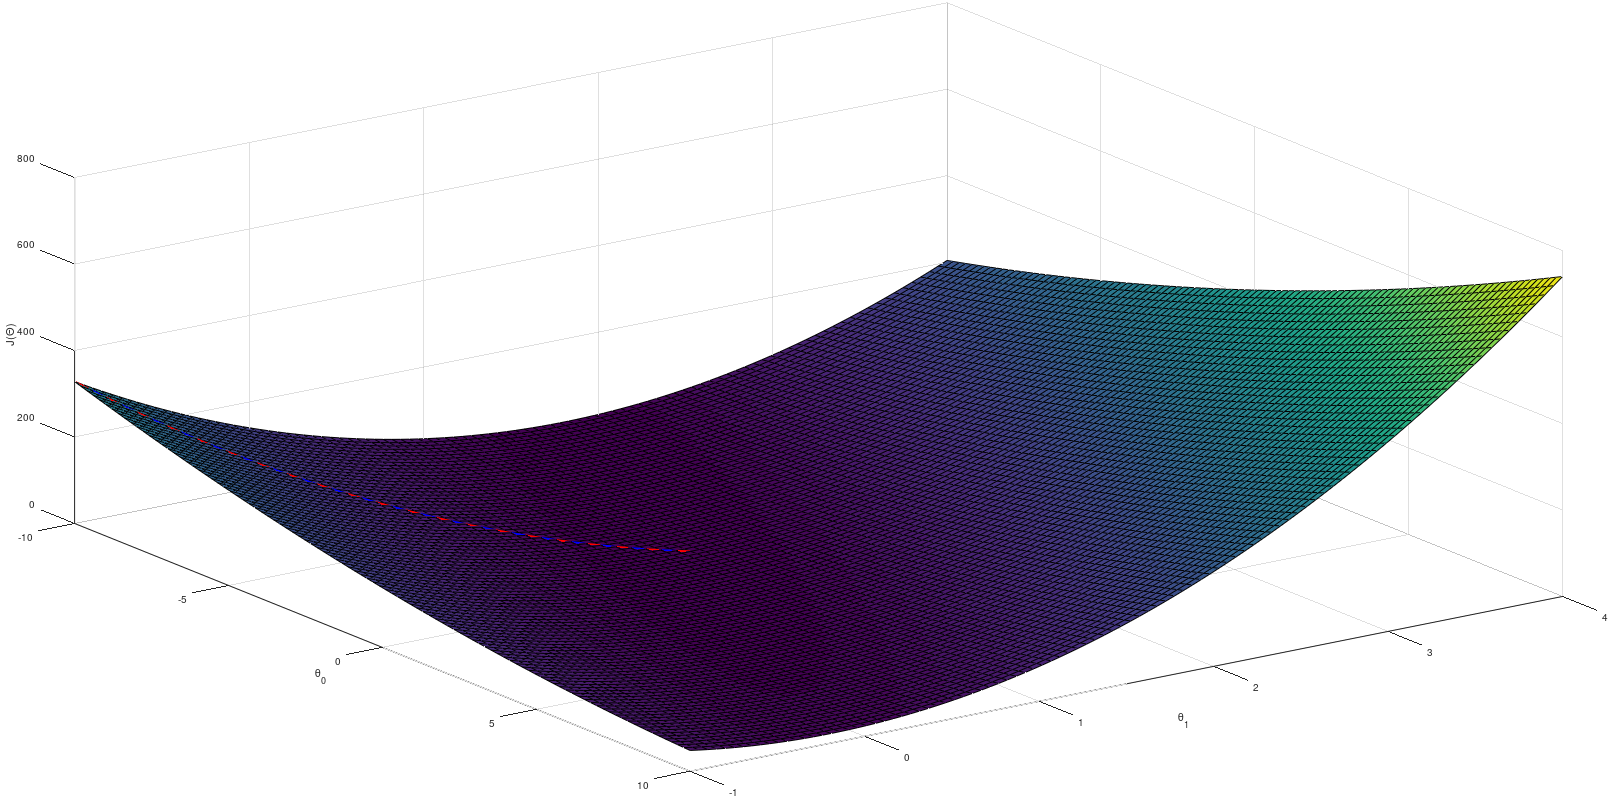
\includegraphics[scale=0.38]{gradientdescent}

\section{Normal equations}
A more analytical way to compute the global minimum of the convex error function is by using normal equations. The normal equation gives the parameters for a minimized error function and is defined as
\begin{center}
\boldmath{$\Theta $}\unboldmath \ $=$ (\boldmath{$X$}\unboldmath$^T$\boldmath{$X$}\unboldmath$)^{-1}$\boldmath{$X$}\unboldmath$^T$\boldmath{$y$}\unboldmath
\end{center}
The theta refers to the matrix containing the minimized \(\theta_j\) values, or weights. The matrix \boldmath{$X$}\unboldmath is the feature dataset, while the matrix \boldmath{$y$}\unboldmath \ is the actual result not predicted by the hypothesis. By taking the squared error function and transform it into a vectorized format:

\[\begin{bmatrix} h_{\boldsymbol{\Theta}} (\boldsymbol{X}^0) - y^0 \\ h_{\boldsymbol{\Theta}} (\boldsymbol{X}^1) - y^1 \\ h_{\boldsymbol{\Theta}} (\boldsymbol{X}^2) - y^2 \\ . \\ . \\ . \\  \\ h_{\boldsymbol{\Theta}} (\boldsymbol{X}^m) - y^m\end{bmatrix}\]

The expression can be split up into two vectors: 
\[\begin{bmatrix} h_{\boldsymbol{\Theta}} (\boldsymbol{X}^0) \\ h_{\boldsymbol{\Theta}} (\boldsymbol{X}^1) \\ h_{\boldsymbol{\Theta}} (\boldsymbol{X}^2) \\ . \\ . \\ . \\ h_{\boldsymbol{\Theta}} (\boldsymbol{X}^m) \end{bmatrix} - \begin{bmatrix} y^0 \\ y^1 \\ y^2 \\ . \\ . \\ . \\ y^m \end{bmatrix}\]
The two vectors can then be simplified, the left one through the identity of the hypothesis function, and the right one given our definition of \boldmath{$y$}\unboldmath:
\[\begin{bmatrix} \boldsymbol{\Theta}^T * \boldsymbol{X}^0 \\ \boldsymbol{\Theta}^T * \boldsymbol{X}^1 \\ \boldsymbol{\Theta}^T * \boldsymbol{X}^2 \\ . \\ . \\ . \\ \boldsymbol{\Theta}^T * \boldsymbol{X}^m \end{bmatrix} - \boldsymbol{y}\]
As the hypothesis function is defined as \(\sum_{i=0}^m \boldsymbol{\Theta}_i x_i\), the vector can be written as:
\[\begin{bmatrix} \boldsymbol{\Theta}_0 * \boldsymbol{X}_0^0 + \boldsymbol{\Theta}_1 * \boldsymbol{X}_1^0 + \boldsymbol{\Theta}_2 * \boldsymbol{X}_2^0 + ... + \boldsymbol{\Theta}_n * \boldsymbol{X}_n^0 \\ \boldsymbol{\Theta}_0 * \boldsymbol{X}_0^1 + \boldsymbol{\Theta}_1 * \boldsymbol{X}_1^1 + \boldsymbol{\Theta}_2 * \boldsymbol{X}_2^1 + ... + \boldsymbol{\Theta}_n * \boldsymbol{X}_n^1 \\ . \\ . \\ . \\ \boldsymbol{\Theta}_0 * \boldsymbol{X}_0^m + \boldsymbol{\Theta}_1 * \boldsymbol{X}_1^m + \boldsymbol{\Theta}_2 * \boldsymbol{X}_2^m + ... + \boldsymbol{\Theta}_n * \boldsymbol{X}_n^m \end{bmatrix} - \boldsymbol{y}\]
The error function can therefore be written as \(\boldsymbol{X\Theta} - \boldsymbol{y}\). To find the square error, the error function can have its terms multiplied by themselves, as so:
\[\frac{1}{2m}(\boldsymbol{X\Theta} - \boldsymbol{y})^T(\boldsymbol{X\Theta} - \boldsymbol{y})\]
Now, to find the minimum \(\boldsymbol{\Theta}\) the expression shall be derived with respect to \(\boldsymbol{\Theta}\) and then solved for \(0\):
\[\frac{\partial}{\partial\boldsymbol{\Theta}}[(\boldsymbol{X\Theta} - \boldsymbol{y})^T(\boldsymbol{X\Theta} - \boldsymbol{y})] = 0\]
The transpose then gets distributed, following the distribution identity \((\boldsymbol{A} + \boldsymbol{B})^T = \boldsymbol{A}^T + \boldsymbol{B}^T\)
\[\frac{\partial}{\partial\boldsymbol{\Theta}}[((\boldsymbol{X\Theta})^T - \boldsymbol{y}^T)(\boldsymbol{X\Theta} - \boldsymbol{y})] = 0\]
Then distributing the parenthesis:
\[\frac{\partial}{\partial\boldsymbol{\Theta}}[(\boldsymbol{X\Theta})^T(\boldsymbol{X\Theta}) - \boldsymbol{y}(\boldsymbol{X\Theta})^T - \boldsymbol{y}^T(\boldsymbol{X\Theta}) - \boldsymbol{y}^T\boldsymbol{y}] = 0\]
Then using the distribution identity again, and collecting like terms given the two vectors are of the same dimensionality:
\[\frac{\partial}{\partial\boldsymbol{\Theta}}[\boldsymbol{X}^T\boldsymbol{\Theta}^T\boldsymbol{X\Theta} - 2\boldsymbol{X}^T\boldsymbol{\Theta}^T\boldsymbol{y} - \boldsymbol{y}^T\boldsymbol{y}] = 0\]
Then splitting the terms and removing the scalar term: 
\[\frac{\partial}{\partial\boldsymbol{\Theta}}[\boldsymbol{X}^T\boldsymbol{\Theta}^T\boldsymbol{X\Theta}] - \frac{\partial}{\partial\boldsymbol{\Theta}}[2\boldsymbol{X}^T\boldsymbol{\Theta}^T\boldsymbol{y}] = 0\]
Evaluating the terms and extracting the scalars:
\[\boldsymbol{X}^T\boldsymbol{X}\frac{\partial}{\partial\boldsymbol{\Theta}}[\boldsymbol{\Theta}^T\boldsymbol{\Theta}] - 2\boldsymbol{X}^T\boldsymbol{y}\frac{\partial}{\partial\boldsymbol{\Theta}}[\boldsymbol{\Theta}^T] = 0 \]
\[2\boldsymbol{X}^T\boldsymbol{X\Theta} - 2\boldsymbol{X}^T\boldsymbol{y} = 0\]
Manipulate the expression with some algebra:
\[2\boldsymbol{X}^T\boldsymbol{X\Theta} = 2\boldsymbol{X}^T\boldsymbol{y}\]
\[\boldsymbol{X}^T\boldsymbol{X\Theta} = \boldsymbol{X}^T\boldsymbol{y}\]
To isolate $\boldsymbol{\Theta}$ the matrix has to be multiplied by its inverse:
\[(\boldsymbol{X}^T\boldsymbol{X})(\boldsymbol{X}^T\boldsymbol{X})^{-1}\boldsymbol{\Theta} = (\boldsymbol{X}^T\boldsymbol{X})^{-1}\boldsymbol{X}^T\boldsymbol{y}\]
\[\boldsymbol{\Theta} = (\boldsymbol{X}^T\boldsymbol{X})^{-1}\boldsymbol{X}^T\boldsymbol{y}\]
\section{The backpropagation algorithm}
Now that the normal equations and gradient descent is explained, the backpropagation algorithm can be explored. The backpropagation algorithm could be thought of as gradient descent in higher dimensions, but in reality backpropagation is simply an addition to gradient descent. Backpropagation is a process, and to give an understanding of what its doing before going into the maths, a timeline for the process would be: 
\begin{center} 1. Perform a feed-forward of the network using training data
\\ 2. Perform backpropagation to get error derivatives w.r.t each weight
\\ 3. Perform minimizing on each weight using derivates
\\ 4. Repeat\end{center}
Backpropagation is an application of the chain rule from calculus. The goal of the algorithm is to get the derivate of every weight and bias with respect to the error function. The derivative permits seeing the impact changing a certain weight has to the overall cost function, along with minimizing the weights with respect to the error function. 


























\end{document}
